\documentclass[conference]{IEEEtran}

\usepackage[utf8]{inputenc}
\usepackage[T1]{fontenc}
\usepackage[english]{babel}
\usepackage{graphicx}
\usepackage{subfig}

\newcommand{\fig}[3][width=\columnwidth]{
  \begin{figure}[ht]
    {\centering{\includegraphics[#1]{fig/#2}}\par}
    \caption{#3}
    \label{fig:#2}
  \end{figure}
	}

\begin{document}

\title{A Cross-layer Approach to Trustfulness in the Internet of Things}

\author{
  \IEEEauthorblockN{Antônio Augusto Fröhlich, Alexandre Massayuki Okazaki,\\ Rodrigo Vieira Steiner, and Peterson Oliveira}
  \IEEEauthorblockA{
	Software/Hardware Integration Lab\\
	Federal University of Santa Catarina\\
	PO Box 476, 88040-900 - Florianópolis, SC, Brazil \\
	{guto,alexadre,rodrigo,peterson}@lisha.ufsc.br\\
  } \and
    \IEEEauthorblockN{\\Jean Everson Martina}
  \IEEEauthorblockA{
	Computer Security Lab\\
	Federal University of Santa Catarina\\
	PO Box 476, 88040-900 - Florianópolis, SC, Brazil \\
	everson@inf.ufsc.br
	}
}

\maketitle

\begin{abstract}
It is a mistake to assume that each embedded object in the Internet of
Things will implement a TCP/IP stack similar to those present in
contemporary operating systems. Typical requirements of ordinary things,
such as low power consumption, small size, and low cost, demand
innovative solutions. %Domain-specific, cross-layer protocols enable
%designers to address such requirements at the same time as they
%incorporate features such as location, timing and security not present
%in the original TCP/IP design. 
In this article, we describe the design,
implementation, and evaluation of a trustful infrastructure for the
Internet of Things based on EPOSMote. The infrastructure was built
around EPOS' second generation of motes, which features an ARM processor
and an IEEE 802.15.4 radio transceiver. It is presented to end users
through a trustful communication protocol stack compatible with TCP/IP.
Trustfulness was tackled at MAC level by extending C-MAC, EPOS native
MAC protocol, with AES capabilities that were used to
encrypt and authenticate IP datagrams packets.  Our
authentication mechanism encompasses temporal information to protect the
network against replay attacks.  The prototype implementation was
assessed for processing, memory, and energy consumption with positive
results.

\end{abstract}

\begin{IEEEkeywords}
Internet of Things; Cross-layer communication protocols; Trustfulness;
\end{IEEEkeywords}

%%%%%%%%%%%%%%%%%%%%%%%%%%%%%%%%%%%%%%%%%%%%%%%%%%%%%%%%%%%%%%%%%%%%%%%%%%%%%%%
\section{Introduction}
\label{sec:intro}
% Context: IoT what we have now and what is there to come
The idea of an Internet of Things (IoT) is quickly materializing through
the adoption of RFID as a replacement for bar code along with the
introduction of Near Field Communication (NFC). We are able to
interface with our daily-life objects over the Internet. However, the next
steps towards a global network of smart objects will drive us through
several large-scale, interdisciplinary efforts. In particular, security
and privacy are issues that must be consistently addressed before IoT
can make its way into people's lives.

% Problem: trustfulness of IoT messages

\emph{Things} in IoT interact with each other and with human beings
through a myriad of communication technologies, often wirelessly, and
subject to interference, corruption, eavesdropping, and
all kinds of attacks. Most of encryption and authentication
techniques was developed for the original Internet---the Internet of People
that we use today---to handle attacks can in theory be applied to the IoT. However, the
microcontrollers used in smart objects will seldom be able to put up
with their requirements. Furthermore, IoT will be subject to particular
conditions not so often faced by today's Internet devices. %Some
\emph{Things} will send messages that will trigger immediate reactions
from the environment.  Capturing and reproducing one such valid message,
even if it is encrypted and signed, could lead complex systems such
as roadways, factories, and even future cities to misbehave. Some
\emph{Things} will harvest energy from the environment for hours before
they can say something to the world. And when they talk, one will have
to decide whether or not to believe in what they say without having a
chance to further discuss the subject (at least not for a couple of
hours). Solutions such as transaction authentication and
channel masking~\cite{Fu:2003} are of little help in this context.

% Solution: of how.

In this paper, we describe the design, implementation and evaluation of
a trustful communication framework for the IoT conceived with these
pitfalls in mind. The framework follows a cross-layer design that
combines medium access control, location, timing, routing and
trustfulness on highly configurable manner. It was evaluated using EPOS'
second generation of motes, EPOSMoteII, which features an ARM processor
and an IEEE 802.15.4 radio transceiver~\cite{EPOSMote}. It is presented
to end users through a trustful communication protocol compatible with
TCP/IP, which per-definition ensures end-to-end reliable and ordered
delivery.  Trustfulness is tackled at MAC level by extending
C-MAC~\cite{Steiner:Sensors:2010}, EPOS native MAC protocol, with
Advanced Encryption Standard (AES)~\cite{AES:2001} capabilities that
were subsequently used to encrypt and authenticate packets. % containing IP datagrams.  
EPOS Precision Time Protocol~(PTP) implementation is used to
enrich the authentication mechanism with temporal information. % protecting against replay attacks.

% Paper organization

Section~\ref{sec:layered} presents the design of EPOS original
communication stack. %, which features layers for each major functionality set.  
EPOS trustful mechanisms are discussed separately in
Section~\ref{sec:trust}. Section~\ref{sec:cross} introduces the new
cross-layer design, in which elements of medium access control,
location, timing, routing, and security are carefully merged in a
single-level protocol.  In Section~\ref{sec:results} we evaluate the new cross-layered protocol on the EPOSMoteII platform,
followed by related works in Section~\ref{sec:related} and 
conclusions in Section~\ref{sec:conclusions}.


%%%%%%%%%%%%%%%%%%%%%%%%%%%%%%%%%%%%%%%%%%%%%%%%%%%%%%%%%%%%%%%%%%%%%%%%%%%%%%%
\section{EPOS Original Communication Protocol Stack}
\label{sec:layered}

EPOS original communication protocols stack features a layered
architecture as suggested by the OSI model. %Each major functionality
%block is implemented in a layer that provides services for upper layers
%using the services provided by the layers bellow.  
Although developed to
be energy efficient and to present low overhead, this architecture is
similar to that of ordinary operating systems traditionally used in the
Internet of People. The original layered architecture is described in
the following sections.
% presented in Figure~\ref{fig:layered_overview} and each of its layers
% are subsequently described.

 % An overview of the original layered architecture is
% presented in Figure~\ref{fig:layered_overview} and each of its layers
% are subsequently described.

\subsection{C-MAC}

C-MAC is a highly configurable MAC protocol for Wireless Sensor
Networks~(WSN) realized as a framework of medium access control
strategies that can be combined to produce application-specific
protocols~\cite{Steiner:Sensors:2010}. It enables application
programmers to configure several communication parameters (e.g.
synchronization, contention, error detection, acknowledgment, packing,
etc) to adjust the protocol to the specific needs of their applications.
%C-MAC's microcomponent framework is driven by a powerful finite-state
%machine that encompasses state transitions found in the most traditional
%MAC protocols for WSN. State machines for several channel polling,
%scheduled contention, and TDMA protocols were first extracted in
%isolation and later merged to produce C-MAC's multiprotocol one.  Each
%of C-MAC's microcomponents is associated with a specific transition in
%that finite-state machine. Customized protocols are then accomplished by
%sorting out inapplicable states. C-MAC's framework is designed so that
%unused microcomponents---that is, those not referred by any transition
%on the customized state machine---simply render their inputs as output.
%C-MAC deploys the same static metaprogramming techniques used in EPOS,
%so this customization procedure is carried out at compilation time and
%thus does not impact the performance of the protocol at run-time. 
An overview of C-MAC is rendered by the activity diagrams of
Figures~\ref{fig:cmac_act_sync}, \ref{fig:cmac_act_send}, and
\ref{fig:cmac_act_receive}.

\fig[scale=.23]{cmac_act_sync}{C-MAC synchronization activity diagram.}
\fig[scale=.23]{cmac_act_send}{C-MAC transmission activity diagram.}
\fig[scale=.23]{cmac_act_receive}{C-MAC reception activity diagram.}

The main configuration points of C-MAC are:

\begin{itemize}

\item \textbf{Physical layer:} These configuration parameters are
  defined by the underlying radio transceiver. %, and usually include
  %parameters such as frequency, transmission power, and data rate.

\item \textbf{Synchronization:} Derived from the mechanisms used to
  exchange synchronization information among nodes. %, including the
  %network duty cycle.

\item \textbf{Collision avoidance:} Configure contention mechanisms used
  to avoid collisions. %, including carrier sense (e.g.  CSMA-CA),
 % programmed contention (e.g. RTS/CTS), or a combination of both.

\item \textbf{Acknowledgment:} Define if and how successful or
  unsuccessful packet exchanges are to be handled.%, including the
%  acknowledgement of preamble packets.

\item \textbf{Error handling:} Determine which mechanisms will be used
  to ensure the consistency of data. % (e.g. CRC).

\item \textbf{Security:} Determine which mechanisms will be used to
  ensure communication security. %, including data encryption and packet
%  authentication.

\end{itemize}

%\fig[scale=.2]{cmac_bmac-packet}{C-MAC packet format when mimicking
%  B-MAC.}

When configured to mimic preexisting MAC protocols %, like B-MAC for instance, 
C-MAC delivers comparable performance. This is due to the use
of static metaprogramming techniques%(e.g. templates, inline functions,
%and inline assembly)
, which ensures that configurability does not come
at the expense of performance or code size~\cite{Steiner:Sensors:2010}.
In this way, C-MAC's instances are fully customized at compile-time and
yield extremely lean run-time MACs. C-MAC high
configurability was essential to the research being presented here. %, for
%it enabled us to customize the MAC protocol to closely match the
%requirements of upper level protocols, and eventually incorporate them.

%Figure~\ref{fig:cmac_bmac-packet} depicts C-MAC packet format when configured to mimic B-MAC.
\subsection{HECOPS}

EPOS location mechanism, the Heuristic Environmental Consideration Over
Positioning System~\cite{Reghelin:MSWIM:2006}, defines a distributed
location algorithm for wireless sensor networks in which every node
estimates its own position after interacting with other nodes. %Only a
%limited number of nodes needs to have exact knowledge of their position coordinates.  
HECOPS establishes a ranking system to determine the
reliability of each estimated position and uses heuristics to reduce the
effects of measurement errors. %, including a scheme to calibrate range
%measurements by comparing, whenever possible, the estimated distance
%with the actual distance between a pair of nodes.  
So far, HECOPS has
been applied in the realm of IoT using two main heuristics: the
relationship between signal degradation and distance inferred from the
Received Signal Strength Indication~(RSSI) provided by
C-MAC~\cite{Pires:INDIN:2008}, and the Time Difference of Arrival~(TDOA)
provided by a UWB transceiver~\cite{Oliveira:SBESC:2012}. The first
heuristic is depicted in Figure~\ref{fig:hecops-overview}. The location
of anchor nodes is determined equipping motes with GPS receivers.

\fig[scale=.25]{hecops-overview}{Overview of HECOPS.}
%\fig[scale=.5]{hecops-packet}{HECOPS packet format.}

\subsection{PTP}

Time synchronization is a mandatory OS feature for many distributed
applications. %In EPOS, we also use network-wide time synchronization to
%improve location estimation and routing, and also to enrich security
%mechanisms with timestamps. 
EPOS timing
protocol~\cite{Oliveira:SBESC:2012} delivers clock time across a
wireless sensor network in conformance with the IEEE 1588 standard, the
Precision Time Protocol~(PTP). A node acting as a master clock extracts
the base time from a GPS receiver and propagates it to slave clocks
following the standard as illustrated by Figure~\ref{fig:ptp-overview}.  Since propagation is usually done by
broadcast or zone multicast, listening nodes take advantage of protocol
interactions to re-calibrate whenever valid PTP messages
are observed in the network. % This feature is accomplished by
%configuring C-MAC to receive PTP packets even if the destination address
%is not that of the listening node. 
This novel kind of clock, which we
named \emph{listener}, adds to masters and slaves while saving
considerable amounts of energy as discussed in
section~\ref{sec:results}.  EPOS PTP is able to keep a PAN synchronized
with sub-millisecond precision.

\fig[scale=.2]{ptp-overview}{Overview of EPOS PTP.}
%\fig[scale=.5]{ptp-packet}{PTP packet format.}

\subsection{ADHOP}

Motes in a wireless sensor network usually propagate data packets in a
multihop fashion and %, most often on a mesh topology and in many cases on an
%all-to-sink strategy. 
IoT devices are likely to follow a similar scheme. %,
%perhaps with networks that will be more segmented and connected to the
%Internet by gateways, but still on a multihop topology. 
In this
scenario, routing will strongly influence performance and energy
consumption. EPOS Ant-based Dynamic Hop Optimization
Protocol~(ADHOP)~\cite{Okazaki:SCPA:2011,Okazaki:Sensors:2012} was
designed to address these questions.  It is a self-configuring, reactive
routing protocol able to handle mobile nodes and to balance energy
consumption across the network. %In the majority of the existing routing
%protocols, whenever a route is considered to be optimal from the
%perspective of the protocols' metrics (usually bandwidth and latency),
%it is intensively reused for the following transmissions. As a result,
%nodes involved in optimal routes tend to exhaust their batteries more
%quickly than other notes, especially in low-power networks, which are
%noisy and error-prone. 
ADHOP is able to handle dynamic topologies with a
combination of heuristics defined around different metrics, thus
adjusting routing according with network needs. ADHOP pheromone
concentration and evaporation rates are dynamically adjusted considering
global information collected and disseminated by ants. %, such as hop
%counting, geographic distance, and round trip time to destination, and
%also using local information about resource availability, including
%residual battery, signal strength, and buffer capacity (see illustration
%in Figure~\ref{fig:adhop-overview}. 
A node forwarding too many packets,
because it is on a strategic location, will adjust pheromone to favor
other routes as soon as it realizes its resources are being drained too
quickly.  For instance, when energy consumption is given a higher
importance by application programmers, ADHOP will adjust pheromone
evaporation rates based on residual energy, eventually demoting a
previously optimal route and consequently balancing energy consumption
across the network.

%\fig[scale=.20]{adhop-overview}{Overview of ADHOP.}
%\fig[scale=.5]{adhop-packet}{ADHOP packet format.}

\subsection{TCP/IP}

TCP is a key protocol for the trustful IoT platform being proposed here,
that ensures ordered delivery of packets. %However, ordinary TCP
%implementations have been tuned for decades to traditional networks,
%made up of wired links and stationary hosts. TCP now performs extremely
%well on such networks. 
Its acknowledgement and flow control mechanisms
have been optimized to efficiently handle congestion, presumably the
unique significant cause for packet loss on low-error rate
networks. In the presence of higher error rates and intermittent
connectivity, %which are typical for IoT wireless links, 
traditional TCP
implementations continue to react to packet losses in the same way,
causing a significant degradation of performance observed by peers as
poor throughput and high latency~\cite{Balakrishnan:1995}.

%EPOS TCP/IP stack was conceived in this context, considering also the
%limited resource availability typical of IoT devices and bearing in mind
%that many \emph{things} will operate on batteries. 
The current EPOS IPv4
implementation uses TCP's window-based flow control mechanism to
implement an \emph{rendezvous} protocol and thus virtually eliminates
buffer management on IoT nodes. The strategy is depicted in
Figure~\ref{fig:tcp-overview-2}. Peers
announce buffer availability for a single message at a time by adjusting
the window length in acknowledgement messages accordingly. Several
optimizations have also been conducted to keep IP datagrams in pace with
IEEE 802.15.4 127-byte MTU. %, a challenging goal for the upcoming IPv6
%version.  
 Energy efficiency is sought in EPOS TCP/IP stack by
incorporating the pheromone concept behind ADHOP as the IP routing
metric.

%\fig[scale=.3]{tcp-overview}{Overview of EPOS TCP/IP.}

\fig[scale=.25]{tcp-overview-2}{Overview of EPOS TCP/IP - Window 0.}

\subsection{Web Services}

Many researchers and practitioners are now talking about a \emph{Web of
  Things} and proposing that our daily objects will be embraced by the Web
using the same protocols of the ordinary Internet. %, including HTTP,
%Corba, SOAP, and RESTful. 
We do not believe that ordinary objects will
ever implement such protocols. %, if not for resources, for the
%impracticability of formally verification such a conundrum.
Nevertheless, in order to be able to design the cross-layer protocol
being proposed here, we concluded that one such an implementation was
necessary. We therefore implemented a small web server for EPOS,
featuring the HTTP and the RESTful protocols, thus enabling our
``things'' to be accessed just like any other web service. Important
here is to observe the enormous overhead represented by the request
message depicted in Figure~\ref{fig:webservice-packet}.

\fig[scale=.45]{webservice-packet}{Message format for a RESTful web service request
  to an EPOSMote.}

%%%%%%%%%%%%%%%%%%%%%%%%%%%%%%%%%%%%%%%%%%%%%%%%%%%%%%%%%%%%%%%%%%%%%%%%%%%%%%%
 \subsection{EPOS  Strategy for Trustfulness}
\label{sec:trust}

IoT devices will often communicate through the air using radio channels
that are open for everyone to peek and poke~\cite{Zhou:2008}. In order
to avoid undesired interference, EPOS devises a trust mechanisms that
adhere the following premises:

\begin{itemize}

\item \textbf{Confidentiality:} the protocol must prevent unauthorized
  access to data.  %It is accomplished by encrypting critical parts of a
  %message before it is transmitted. 
  As receivers must have the right key to
  decrypt it. This calls for a key management strategy.

\item \textbf{Authenticity:} the protocol must be able to confirm the
  origin of a message. %It is accomplished by authenticating the
%  message by the means of a message authentication code~(MAC) generated by a
%  keyed hash function.

\item \textbf{Integrity:} the protocol must ensure that the message was
  not modified on the way from sender to the recipient. % It is
%  accomplished with a keyed checksum.

\end{itemize}

We believe that security must be handled at the lowest possible level in
the system, since each additional layer of software can potentially make
room for exploits. Therefore, we incorporated the proposed trustfulness
mechanism into C-MAC. It was accomplished through the addition of new
states to C-MAC's finite-state machine and the corresponding
microcomponents to its framework. These elements were already present at
Figures~\ref{fig:cmac_act_send} and~\ref{fig:cmac_act_receive} in
Section~\ref{sec:layered}.  \texttt{ENCRYPT} is responsible for
encrypting the payload.  \texttt{SIGN} attaches the time-stamp, which is
also encrypted, and the message authentication code to the packet.
\texttt{DECRYPT} decrypts the payload, while \texttt{AUTHENTICATE}
verifies if both the time-stamp and authentication code are valid.

\subsubsection{Key Management}

For key management, we opted for a centralized key distribution scheme.
%as shown in Figure~\ref{fig:key_management}. 
Each sensor shares a
symmetric key with the gateway, which is kept in secret by both. % (i.e. it
%is never transmitted clear over the network). 
These symmetric keys are
generated following a Diffie–Hellman scheme %, in which two parties that
%have no prior knowledge of each other jointly establish a shared secret key 
over insecure communications channel~\cite{Diffie:1976}. We use EPOS' secure key bootstraping scheme as shown on Figure~\ref{fig:EPOS_Secure_start}.

Our secure key bootstraping protocol enables EPOSmotes to be deployed and keyd securely at a later stage. 
The protocol's requirements are that the gateway knows the serial number of the nodes he will be sharing keys with,
and that the nodes are able to synchronize time, thus enabling the use of an one-time password generation scheme. Both assumtions are easely achievable 
using our framekwork infrastructure.

We assume that most of communication in an IoT scenario will occur
between devices and the gateway, but devices willing to interact with
each other directly have the option to ask the gateway for a temporary
group key. Alternatively, sporadic device-to-device communication can be
handled by the gateway on a store-and-forward scheme.

%\fig[scale=.3]{key_management}{Overview of key management in EPOS.}
\fig{EPOS_Secure_start}{Overview of key management in EPOS.}

\subsubsection{Replay Attacks}

To countermeasure replay attacks %, that is, to prevent a captured message
%to be improperly reused a second time, 
we added a time-stamp to C-MAC's
packets. The engines generating time-stamps across the network are kept
synchronized via our PTP implementation. Master
clocks are usually gates and produce time seeds based on a GPS receiver
or similar device. %Time-stamps enable the protocol to discard a message
%that was reused.
%eavesdropped by an observer and used later in an attack.

\subsubsection{Message Authentication Code}

The ZigBee specification of high level protocols for IEEE 802 personal
area networks defines a security architecture that is closely related to
the Advanced Encryption Standard~(AES)~\cite{ZIGBEE}. This has pushed
manufacturers to include AES hardware accelerators into many IEEE
802.15.4 platforms. % and establishes a guideline for security-related
%research in the area. 
We therefore considered two AES-based Message
Authentication Code~(MAC) for EPOS: Counter with CBC-MAC (CCM), which is
a generic authenticated encryption block cipher mode for AES~\cite{CCM};
and Poly1305-AES, a state-of-the-art computes a 16-byte authenticator of
a variable-length message using a 16-byte AES key, a 16-byte additional
key, and a 16-byte nonce~\cite{Bernstein:2005}.

\subsubsection{Trusted Packets}

%Figure~\ref{fig:trust-format} depicts the format of an EPOS trustedpacket.
Each packet includes the protocols headers, the application
data, a time-stamp representing the current network time delivered by
PTP, and the MAC produced using the AES accelerator. The application
data is encrypted along with the time-stamp. Since the shared key used
by AES was negotiated directly with the gateway, decrypting a valid
message immediately renders the sender's identity.

%\fig[scale=.3]{trust-format}{EPOS trusted packet format.}

%\subsection{Stack}

%EPOS communication protocol stack arises from the combination of the
%elements discussed so far in this section. It is show in
%Figure~\ref{fig:layered_stack-bmac}.

%\fig{layered_stack-bmac}{EPOS original communication protocol stack.}

%%%%%%%%%%%%%%%%%%%%%%%%%%%%%%%%%%%%%%%%%%%%%%%%%%%%%%%%%%%%%%%%%%%%%%%%%%%%%%%
\section{Cross-layer Protocol}
\label{sec:cross}

After having implemented EPOS protocol stack piece by piece over almost
a decade, we observed that the traditional layered design % established by the OSI model and partially present in most 
of the contemporary
communication stacks was inducing a lot of data replication on different
layers. % and also a lot of duplicate communication among layers. 
Compelled
by the necessity of designing a communication protocol stack for the
Internet of Things that could match its requirements of low overhead and
low power, we reorganized C-MAC's microcomponent framework to combine
aspects of medium access control, location, timing, routing, and
trustfulness on a highly configurable cross-layer protocol.

The proposed cross-layer protocol exploits two characteristics of
the original stack responsible for most of the overhead:

\begin{itemize}

\item \textbf{Information Sharing:} Status information about the local
  node and about its interactions are used across several
  layers. Energy availability, residual memory, transmitted and received
  packets, locally known address mappings are some examples of status information
  intensively used by several layers. Storing it separately and
  requesting in on the demands of a single layer is a major source of
  overhead. We opted for a single shared table containing all the
  information. % used by the protocols.

\item \textbf{Implicit Learning:} The information locally handled by a
  node about its current status and that of its neighbors can be
  implicitly update %on a number of occasions. 
  For instance, acknowledge
  and beacon messages can carry location, timing, and routing
  information almost for free. This kind of information %, along with
  %locally obtained elements such as energy and RSSI, 
  can be updated on
  each received message, thus preventing message exchanges originally
  conceived to obtain them.
\end{itemize}

We took advantage of these observations while designing the low-overhead
cross-layer protocol. We first combined several pieces of the original
finite-state machines to incorporate the behavior of each layer and
subsequently adjusted the format of packets to incorporate the
corresponding data. The result is depicted in
Figure~\ref{fig:cmac_rbmac-packet}.

\fig[scale=.3]{cmac_rbmac-packet}{EPOS cross-layer protocol stack from the perspective
  of packet format.}

%%%%%%%%%%%%%%%%%%%%%%%%%%%%%%%%%%%%%%%%%%%%%%%%%%%%%%%%%%%%%%%%%%%%%%%%%%%%%%%
\section{Evaluation}
\label{sec:results}

We gauged the proposed cross-layer protocol by comparing it to the
original protocol stack of EPOS. % in terms of both performance and
%resource consumption. 
The conceived experiments were carried out on
EPOSMoteII atop of OpenEPOS 1.0. Whenever simulation was needed, OMNeT++
was used with a realistic model. The following sections discuss relevant
details of both scenarios, EPOSMote and the simulation model. %, to sustain
%the results that are present just afterwards.

\subsection{EPOSMote}

The EPOSMote is an open hardware project~\cite{EPOSMote}. The project
main objective is delivering a hardware platform to allow research on
energy harvesting, biointegration, and MEMS-based sensors. The
EPOSMoteII platform focus on modularization, and thus is composed by
interchangeable modules for each function. Figure
\ref{fig:emote2-picture} shows the development kit which is slightly
larger than a R\$1 coin.

\fig[scale=.065]{emote2-picture}{EPOSMoteII SDK side-by-side with a R\$1 coin. %On
 % the left the sensing module. On the right the main module.
 }

Figure \ref{fig:emote2-block_diagram} shows an overview of the EPOSMoteII
architecture. Its hardware is designed as a layer architecture composed
by a main module, a sensing module, and a power module. The main module
is responsible for processing, storage, and communication. The model
used in this research features a 32-bit ARM7 processor, 128kB of flash,
96kB of RAM, and an IEEE 802.15.4-compliant radio transceiver. %We have
%developed a startup sensing module, which contains some sensors (e.g.
%temperature and accelerometer), leds, switches, and a micro USB (that
%can also be used as power supply).

\fig[scale=.4]{emote2-block_diagram}{Architectural overview of EPOSMoteII.}

\subsection{Simulation Model}

OMNeT++ simulator is an extensible, modular, component-based C++
framework for building network simulations. %, and it is useful while modeling wireless communication. 
Table~\ref{tab:omnet} shows the OMNeT++
simulation parameters used for the IEEE 802.15.4 simulated network. In
these experiments, each simulation scenario ran for 900 seconds in an
environment of high mobility that is conducive to high data loss. The
simulation places nodes randomly in a squared area of $1.44~km^2$ (edges
of twelve hundred meters), and each node moves at a maximum speed of
five meters per second, according to the Mass Mobility
algorithm~\cite{Perkins:1999}. Twenty mobile source nodes generates data
traffic to other twenty mobile sink nodes. The experiment explores the
behavior of ADHOP varying the heuristic information and the number
of nodes, ranging from twenty to two hundred. We compare it with
AODV and AOER algorithms for data delivery ratio and energy
consumption.

\begin{table}[h]
\centering
\caption{OMNeT++ Configuration}
\label{tab:omnet}
\begin{tabular}{l|r}
\hline \hline
\multicolumn{2}{l}{\bf{Parameter}}  \\
\hline
Simulation Time               & $900~seconds$     \\
Number of Nodes               & $20 \sim 200$     \\
Area                          & $1200m~X~1200m$   \\
Mobility Model                & $Mass~Mobility$   \\
Application Message Length    & $56~bytes$        \\
Application Message Frequency & $0.25~Hz$         \\
ADHOP Header Length           & $6~bytes$         \\
PHY Transmitter Power         & $1~mW$            \\
PHY Sensitivity               & $-85~dBm$         \\
PHY Thermal Noise             & $-110~dBm$        \\
Channel Carrier Frequency     & $2.4~GHz$         \\
Battery Voltage               & $3~V$             \\
Battery Capacity              & $2~mAh$           \\
\hline
\end{tabular}
\end{table}

\subsection{Results}

We gauged the implementation of the trustful IoT infrastructure proposed
in this paper in respect to three aspects: memory consumption,
encryption/decryption time, and energy consumption. For all experiments,
we used GCC 4.4.4 to compile the application and the run-time support
system (i.e. EPOS). EPOSMoteII ARM processor clock was set to 24 MHz.
Messages were adjusted to carry a payload of 16 bytes when encryption
was activated and 7 (request) and 6 (reply) bytes otherwise. EPOSMoteII
radio transceiver was adjusted to transmit at 4.5 dBm.

%Figure~\ref{fig:test_scenario} illustrates our test scenario. We used
%two EPOSMoteII.  
One node acts as a base station for the local IoT,
interfacing its nodes to the ordinary Internet\footnote{For a larger
  scale experiment, the gateway would rather be configured to provide
  some sort of NAT service between both realms, thus alleviating the
  address limitation of IPv4.}, while the other one is a sensor node.
The base station broadcasts encrypted temperature requests every 10
seconds. The sensor node decrypts the request, collects the required
data, and sends back a signed and encrypted reply.

%\fig[scale=.5]{test_scenario}{Trustful IoT infrastructure evaluation scenario.}

%%%% review this paraghaph, encryption is not done at application any more
In order to obtain the memory footprint of our implementation, we used
the \texttt{arm-size} tool that is part of GNU Binutils. Results are
shown in Table~\ref{tab:CodeSize}. The \textit{AES mediator} column
represents the code needed to interact with the AES hardware accelerator
%available on EPOSMoteII 
in order to accomplish encryption, decryption,
and authentication.  \textit{App using AES} column presents the code
size of the application using the proposed trusted infrastructure and
the \textit{App without AES} column the size when using the original,
plain text, TCP/IP stack. It is possible to notice that there is a
difference between the value of \textit{App using AES} and the sum of
\textit{App without AES} and \textit{AES mediator}. This is due to the
fact that not all methods from the \textit{AES mediator} are used in
\textit{App using AES}. Mediator methods that are not effectively
invoked by the client program are eliminated during compilation.  This
is due to the fact that besides including the mediator code the
\textit{App using AES} has to call this code, so it can be executed,
whereas \textit{App without AES} has no such calls.

\begin{table}[htb] % [htb]-> here, top, bottom
  \centering   % tabela centralizada
  \setlength{\arrayrulewidth}{2\arrayrulewidth}  % espessura da linha
  \setlength{\belowcaptionskip}{10pt}  % espa\c{c}o entre caption e tabela
  \caption{Memory footprint.}
  \begin{tabular}{|c|c|c|c|} % c=center, l=left, r=right 
    \hline
    \multicolumn{1}{|c|}{\textbf{Section}} & \multicolumn{1}{|c|}{\textbf{AES mediator}} & \multicolumn{1}{|c|}{\textbf{App using AES}} & \multicolumn{1}{|c|}{\textbf{App without AES}}\\
    \hline \hline
    .text & 1336 bytes & 47184 bytes & 45916 bytes \\
    \hline
    .data & 0 bytes & 217 bytes & 217 bytes \\
    \hline
    .bss  & 10 bytes & 5268 bytes & 5268 bytes \\
    \hline
    TOTAL & 1346 bytes & 52669 bytes & 51401 bytes \\
    \hline
  \end{tabular}
  \label{tab:CodeSize}
\end{table}

We used an oscilloscope to measure the time needed to encrypt, decrypt
and authenticate messages in our infrastructure. A General Purpose
Input/Output (GPIO) pin in EPOSMoteII is connected to the oscilloscope.
%and set to high before the intended procedure is executed and reset to
%low right after. 
We run the experiments for one minute and calculated
the averages shown in Table~\ref{tab:ProcessingTime}. Obtained values,
besides confirming the efficiency of the implementation in terms of
execution time, also have a positive impact in the node's battery
lifetime.

\begin{table}[htb] % [htb]-> here, top, bottom
  \centering   % tabela centralizada
  \setlength{\arrayrulewidth}{2\arrayrulewidth}  % espessura da linha
  \setlength{\belowcaptionskip}{10pt}  % espa\c{c}o entre caption e tabela
  \caption{Encryption/decryption/MAC check processing time.}
  \begin{tabular}{|c|c|c|c|} % c=center, l=left, r=right 
    \hline
    \multicolumn{1}{|c|}{\textbf{}} & \multicolumn{1}{|c|}{\textbf{Encryption}} & \multicolumn{1}{|c|}{\textbf{Decryption}} & \multicolumn{1}{|c|}{\textbf{MAC Check}} \\
    \hline \hline
    Time & 17 $\mu$s & 15 $\mu$s & 12 $\mu$s \\
    \hline
  \end{tabular}
  \label{tab:ProcessingTime}
\end{table}

%%%From Guto to Rodrigo: extrapolar para 1 hora!
Figure~\ref{fig:energy} shows the energy consumed by both applications%,with and without AES, 
over the time. The small increase in energy
consumption for \textit{App using AES} arises from the efficient usage
of the hardware accelerator.% available in EPOSMoteII. 
After 10 minutes
executing, the difference is minimal (53.2 J with AES and 52.6 J
without), and after 1 hour, the applications have consumed 319.5 J and
315.5 J, respectively, a difference of 1.25\%.

\fig{energy}{Energy consumption.}

%%%ADHOP Results

The energy efficiency, shown in Figure~\ref{relation} in logarithmic
scale, is the division of the overall energy consumption by the amount
of packets successfully delivered. % in a network environment. 
Energy-Aware
ADHOP (EA-ADHOP) routing algorithm produces better results in terms of
energy efficiency than ADHOP, AODV, and AOER. We can notice that this
approach can improve energy use while reducing the energy consumption
and enhancing data delivery ratio. This differs from AOER, which has an
aggressive method to reduce the energy consumption \cite{Shuang:2009},
%thus affecting the data delivery ratio, 
as shown in
Figure~\ref{data_packet_delivery_ratio}. This adds to the low bit rate
of IEEE 802.15.4 nodes, making the connectivity worse in higher speeds
\cite{Zen:2008}. This means greater competition for the medium implying
in collisions, congestions, data loss, and greater energy consumption
for mobile, dense, and scalable networks, causing the depletion of
energy on the routes.

\begin{figure}[h]
\centering
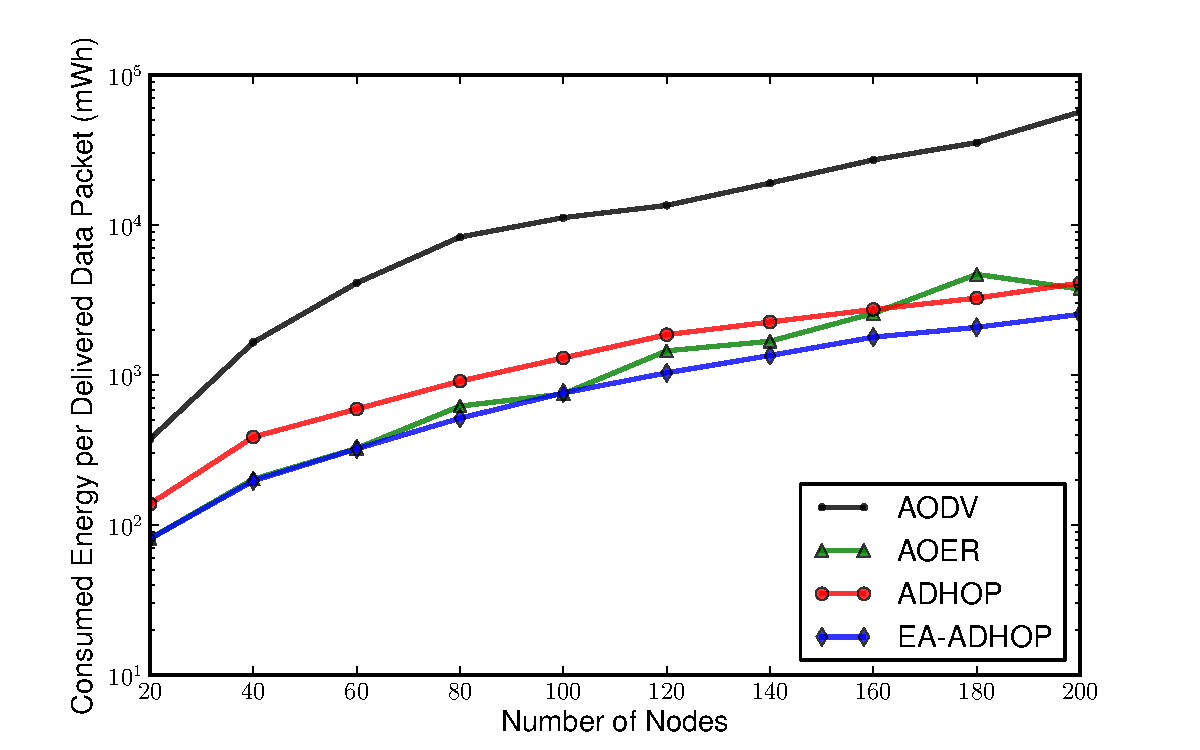
\includegraphics[width=.85\columnwidth]{fig/relation.pdf}
\caption{Energy Consumption per Delivered Data.}
\label{relation}
\end{figure}

\begin{figure}[h]
\centering
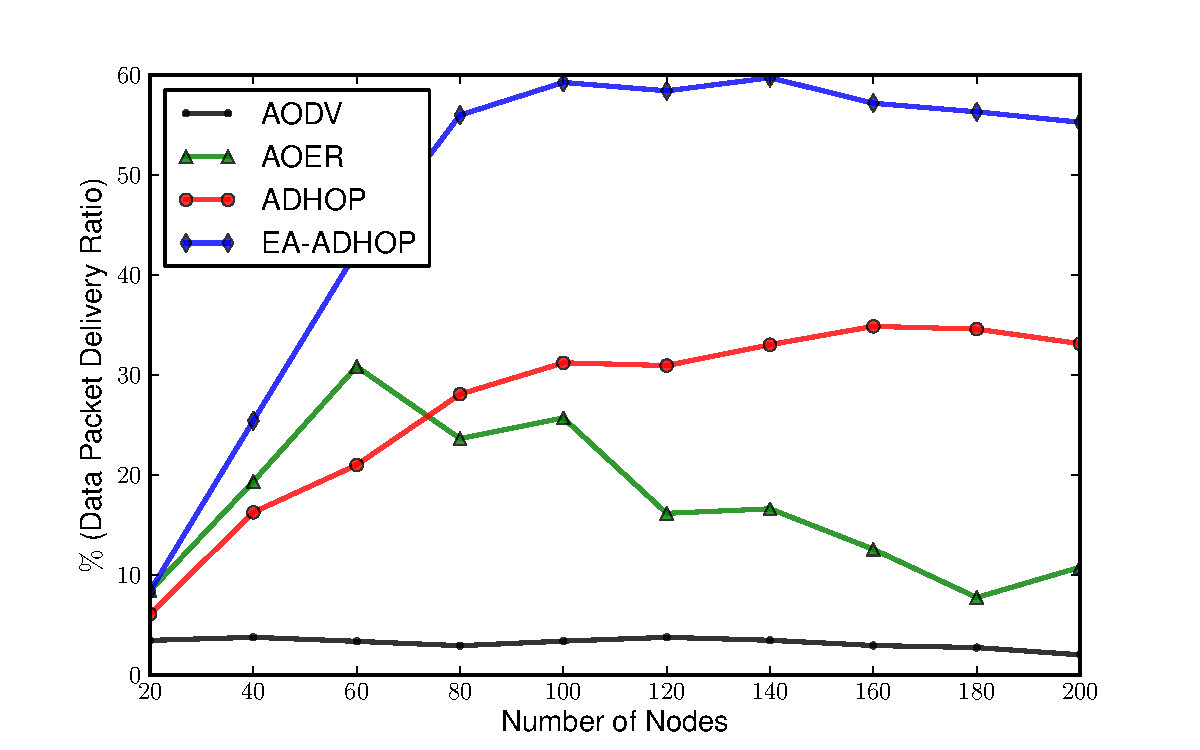
\includegraphics[width=.85\columnwidth]{fig/data_packet_delivery_ratio.pdf}
\caption{Delivery Ratio of Data Packets.}
\label{data_packet_delivery_ratio}
\end{figure}

Another important characteristic of ADHOP is shown in
Figure~\ref{routing_overhead}. Route Requests, Route Replies, and Route
Errors are message types defined by AODV. %Each time a route breaks,
%AODV flood the network with these messages to notify and/or define a new
%route. Such behavior explains the low data delivery ratio of AODV. 
In
ADHOP, data is sent along with the ants thereby decreasing the
amount of control packets in the network. Accordingly, our approach
tends to produce low routing overhead for sparse networks due to low
connectivity. However, it also produces high link failures, shown in
Figure~\ref{link_failures}. We can notice that ADHOP, AODV, and AOER
produce better results of link failures than EA-ADHOP. Since this
approach aims at energy efficiency instead of connectivity, the links
between neighbor nodes tend to be more susceptible to failures.


\begin{figure}[h]
\centering
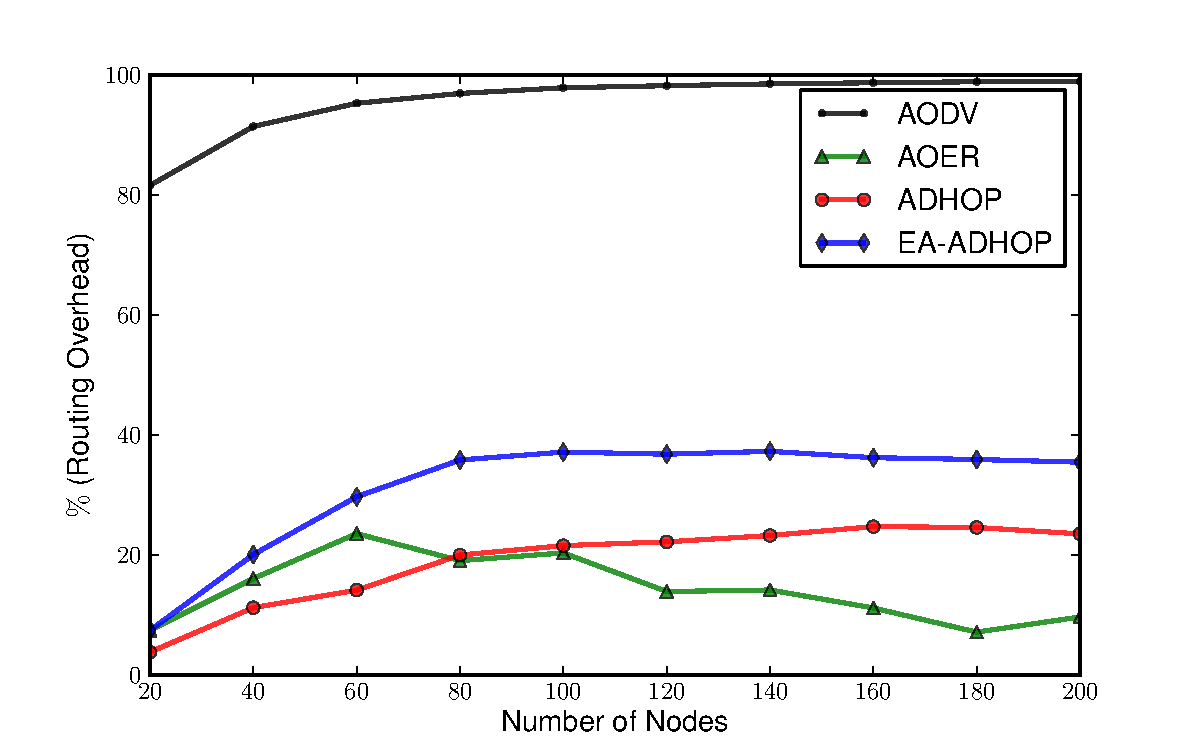
\includegraphics[width=.85\columnwidth]{fig/routing_overhead.pdf}
\caption{Overhead for the maintenance of the routing mechanism.}
\label{routing_overhead}
\end{figure}

\begin{figure}[h]
\centering
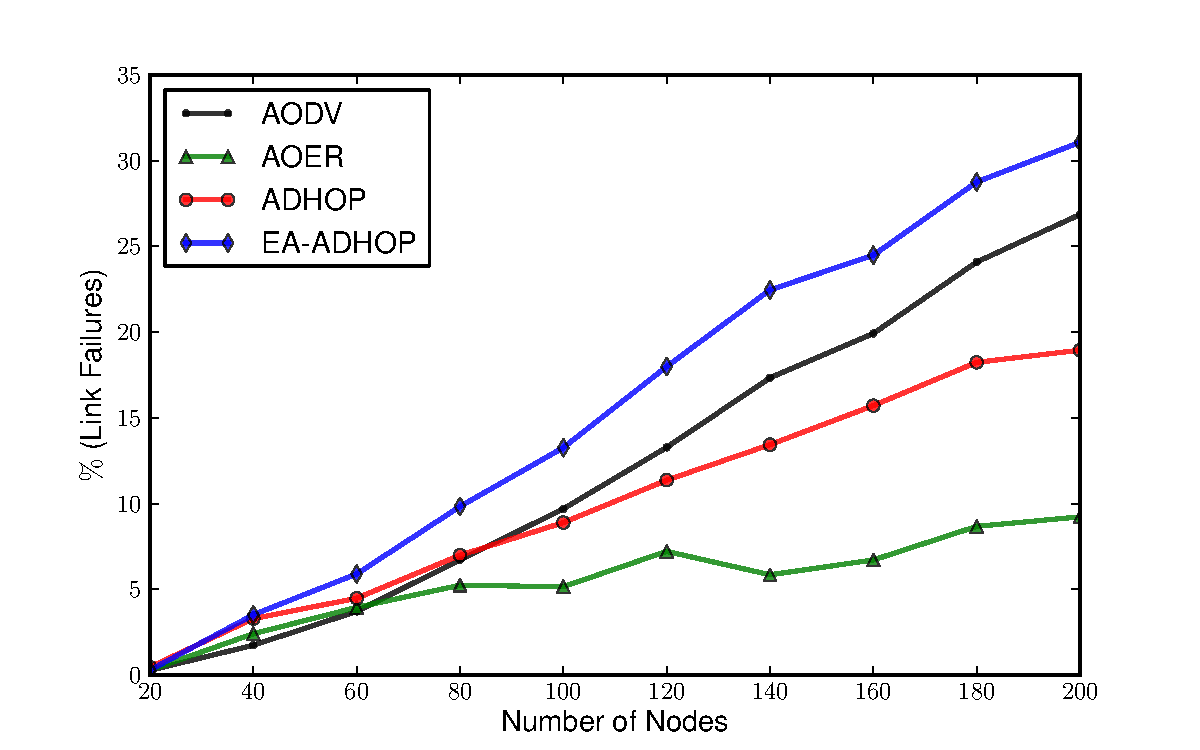
\includegraphics[width=.85\columnwidth]{fig/link_failures.pdf}
\caption{Link Failures}
\label{link_failures}
\end{figure}
%%%%%%%%%%%%%%%%%%%%%%%%%%%%%%%%%%%%%%%%%%%%%%%%%%%%%%%%%%%%%%%%%%%%%%%%%%%%%%%
\section{Related Work}
\label{sec:related}

TinySec~\cite{Karlof:2004} defines a link-layer security architecture
for Wireless Sensor Networks (WSNs). %, providing encryption and authentication. 
TinySec supports two different security options:
authenticated encryption (TinySec-AE), and authentication only
(TinySec-Auth). In authenticated encryption mode, TinySec encrypts the
data payload according to the Skipjack block cipher~\cite{Skipjack:1998}
and authenticates the packet with a Message Authenticity Code (MAC). %The
%MAC is computed over the encrypted data and the packet header. 
In
authentication only mode, TinySec authenticates the entire packet with a
MAC, but the data payload is not encrypted. The inclusion of a MAC to
ensure the authenticity and integrity have a cost on radio usage and,
consequently, in energy consumption. This is because the hash values
commonly represent a long sequence of bits. %---the length of a MAC
%determines the security strength of a MAC function~\cite{Sun:2010}.
TinySec achieves low energy consumption by reducing the MAC size, hence
decreasing the level of security provided. TinySec also does not attempt
to protect against replay attacks, and does not discuss how to establish
link-layer keys.  TinySec was implemented in TinyOS and runs on Mica,
Mica2, and Mica2Dot, each using Atmel processors. TinySec
has 3000 lines of nesC code~\cite{Gay:2003} and the implementation
require 728 bytes of RAM and 7146 bytes of space.

MiniSec~\cite{Luk:2007} is a secure network layer protocol for WSNs
which attempts to solve the known problems of TinySec. %MiniSec
%accomplishes this by combining three techniques. 
First, it employs a
block cipher mode of operation that provides both privacy and
authenticity in only one pass over the message data. Second, MiniSec
sends only a few bits of the Initialization Vector~(IV) %---a block of
%bits used by some operating modes to randomize the encryption, producing
%distinct ciphertexts from the same plaintext over time---
while retaining
the security of a full-length IV per packet. In order to protect against
replay attacks and reduce the radio's energy consumption, it uses
synchronized counters. %, but only sending the last bits of the counter
%along with each packet. 
However, \textit{Jinwala et al.} showed that
such scheme requires costly resynchronization routines to be executed
when the counters shared are desynchronized (packets delivery
out-of-order)~\cite{Jinwala:2009}.

Focusing on sensor battery's useful life, \textit{Braun and
  Dunkels}~\cite{Braun:2007} introduces an approach to support energy
efficient TCP operation in sensor networks. The concept called TCP
Support for Sensor nodes (TSS) allows intermediate sensor nodes to cache
TCP data segments and to perform local retransmissions % when they assume
%that a cached segment has not been received by the successor node
%towards the destination, by not receiving an acknowledgement packet. 
TSS
does not require any changes to TCP implementations at end points, and
simulations show that it reduces the number of TCP data segment and
acknowledgement transmissions in a wireless network.
\textit{Ganesh}~\cite{Ganesh:2009} also introduces a mechanism
which improves TCP performance, called TCP Segment Caching.

\textit{Elrahim et al.}~\cite{Elrahim:2011} proposes an
energy-efficient way to implement TCP protocol in scenarios with high
losses. They present a modified Congestion Control Algorithm for WSN.
%Since a TCP sender constantly tracks the Round Trip Time (RTT) for its
%packets, and uses a timeout mechanism to trigger retransmissions in case
%an ACK is not received before expiration. 
By increasing 
retransmission timeout value, they reduce the number of TCP segment
transmissions that are needed to transfer a certain amount of data
across a wireless sensor network with relatively high bit/packet error
rates.

The size of TCP implementation also is important when developing
for resource-constrained sensors. NanoTCP~\cite{Jardak:2008} is a
protocol stack for WSNs with reduced overhead. The low memory
consumption of the protocol show its suitability to resource constrained
devices. But nanoTCP is a simplified version of TCP protocol, not being fully compatible.  However, other
implementations such as uIP and lwIP faithfully represent the TCP
protocol. %uIP intended for tiny microcontroller systems where code size
%and RAM are severely constrained, and it requires 4-5 kilobytes of
%code space and a few hundred bytes of RAM. The other TCP stack, lwIP, is
%larger than uIP, but provides better throughput.%~\cite{citar uIP e lwIP:http://www.sics.se/~adam/software.html}.

Huai proposes to cut down duty cycles and decrease the energy
consumption of executing the AES algorithm by running both CTR and
CBC-MAC in parallel~\cite{Huai:2009}. Similarly to our scheme, their
design employs a hardware accelerator to offload CPU. It uses an 8-bit
data path and a shared key expansion module with both AES cores,
encryption and authentication. They achieved an encryption time of 71.6
ns for a payload of 17 bytes. Their parallel hardware acceleration
provides better results when compared with the sequential AES hardware
accelerator in the FreeScale MC13224V present in EPOSMoteII. %On the
%other hand, Lee evaluated the performance of AES-128 CBC on an 8-bit
%microcontroller~\cite{Lee:2010}. Time and CPU cycle grew proportionally
%to payload size, reaching 449 ms to encrypt and 456 ms to decrypt 16
%bytes of data.

Furthermore, this paper analyses communication efficiency through
the total delay per hop, and it shows that when the scale of the sensor
networks grows, the delay has been doubled, and energy consumption has
also increased accordingly.

%%%%%%%%%%%%%%%%%%%%%%%%%%%%%%%%%%%%%%%%%%%%%%%%%%%%%%%%%%%%%%%%%%%%%%%%%%%%%%%
\section{Conclusions}
\label{sec:conclusions}

This paper presented a trustful infrastructure for the IoT developed
within the realm of project EPOS. By trustful, we mean \emph{reliable}
and \emph{secure}.  Aspects such as people privacy and data dependability have not been considered in this
paper.  The proposed infrastructure is implemented around the EPOSMoteII
platform and delivered to end users through a trustful communication
protocol stack compatible with TCP/IP. Trustfulness for the
infrastructure was achieved through a combination of mechanisms. From
TCP/IP, we inherited reliable and ordered end-to-end packet delivery.
C-MAC was enriched with AES-based encryption and authentication. It now
also time-stamps messages to prevent replay attacks.  Authentication is
performed using a centralized key distribution scheme in which each
sensor shares a unique key with the local base station. We also developed a secure key bootstraping for key agreement between nodes and gateways. We
experimentally evaluated our proposal in terms of memory consumption,
encryption/authentication time, and energy consumption. The results
confirm that the proposed infrastructure is able to provide
confidentiality, authentication, integrity, and reliability without
introducing excessive overhead to a network of things, a key step in
making the Internet of Things a daily reality.

\bibliographystyle{plain}
\bibliography{wsn,lisha}

\end{document}
